%%%%%%%%%%%%%%%%%%%%%%%%%%%%%%%%%%%%%%%%%%%%%%%%%%%%%%%%%%%%%%%%%%%%
% Diskussion und Ausblick
%%%%%%%%%%%%%%%%%%%%%%%%%%%%%%%%%%%%%%%%%%%%%%%%%%%%%%%%%%%%%%%%%%%%

\chapter{Logik Lehrtools mit React}\label{Lehrtools}
Dieses Kapitel enthält den eingangs erwähnten zweiten Teil dieser Arbeit, das Logik-Lehrtools-Projekt. Dieser zweite Teil ist aufgeteilt in die Teilaufgaben die das Projekt beinhaltet. Zunächst wird über ein Ablaufdiagramm gezeigt wann die einzelnen Komponenten bei der Nutzung zusammenspielen. Anschließend werden diese Komponenten detailliert aufgeführt und ihre Rolle im Ablauf dargelegt. Ebenso werden Entscheidungen und Probleme der Projektdurchführung erläutert. Zuerst werden hier die durchgeführten Anpassungen am bereits vorhandenen Java-Programm erklärt. Anschließend folgen die zwei Webentwicklungskomponenten: der verwendete Webserver und die React-Applikation. Abschließend dann die Server-Schnittstelle, die die Kommunikation zwischen Webseite und Java-Programm regelt.
\pagebreak
\section{Ablauf}
In Abbildung 4.1 ist der Ablauf vom Aufruf der Seite bis zur Anzeige der Resultate dargestellt. Deutlich sichtbar ist, wie nach den ersten beiden Schritten die Kommunikation nicht mehr über den Webserver abläuft. Stattdessen wird die neben dem Server laufende API nunmehr zentral für den Austausch.
\begin{figure}[H]
     \centerline{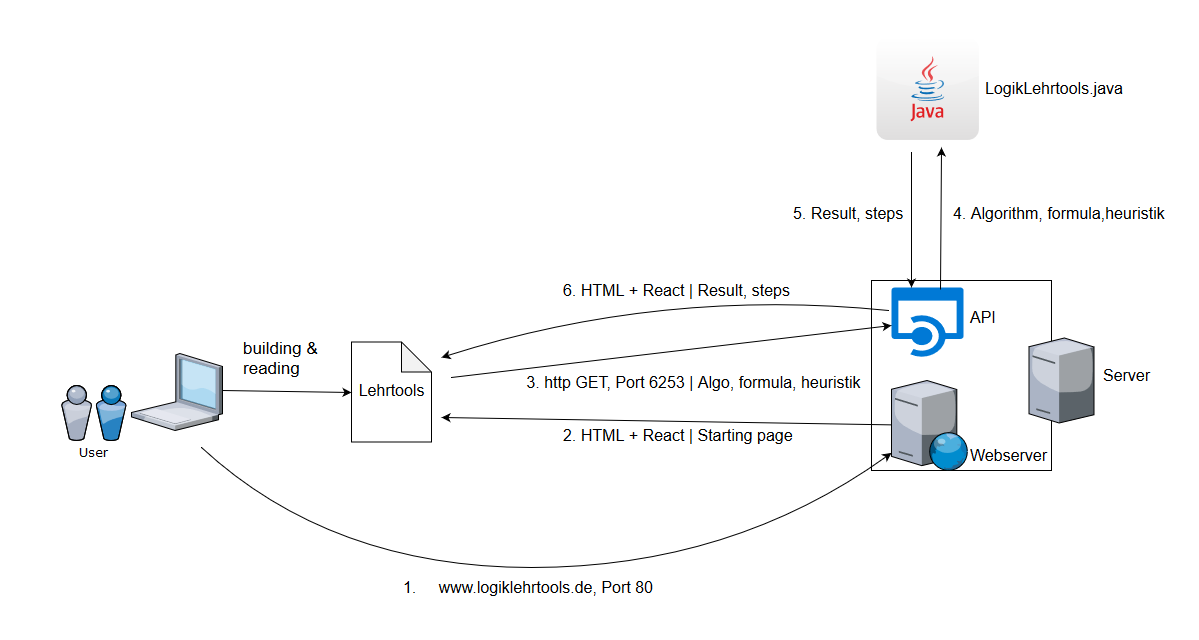
\includegraphics[width=15cm]{../Abbildungen/AblaufLehrtools.png}}
  \caption{Ablauf der Anwendung}
  \label{fig1_1}
\end{figure}
\section{Anpassung der Java Software}
Um das bereits vorliegende Java-Programm von Herrn Espinoza verwenden zu können waren einige Modifikationen daran notwendig. Herr Espinoza hatte seine Applikation mit Benutzeroberfläche entworfen und die logischen Abläufe an eine solche angepasst. Die Aktionen der Applikation wurden alleinig durch die Zustände und Nutzeraktionen dieser Benutzeroberfläche gesteuert. Während das für ein Standalone-Programm durchaus sinnvoll war, warf es Schwierigkeiten für die Webapplikation auf. Sind die Aktionen einer Webapplikation von früheren Aktionen oder Inputs abhängig, so ist  eine sehr viel größere Menge an Kommunikation zwischen Server und Client nötig, ebenso wie eine komplexere Benutzeroberfläche und ein höheres Maß an Handlungen der Nutzer. \\
Für dieses Projekt war eine stateless Implementierung besser geeignet, da die Grundidee des Tools die Anwendung verschiedener Algorithmen war. Bei einer solchen Implementierung ist das Output nur vom Input und nicht von verschiedenen Zuständen abhängig. Die festen Regeln, denen Anwendung und Darstellung der Algorithmen folgen, werden so durch eine solche Implementierung widergespiegelt.\\
Einzelne Funktionen, wie das stete Wählen der nächsten Resolutionsvariable und die Möglichkeit im Algorithmus einen Schritt zurück zu gehen, wurden daher entfernt. Stattdessen ist nun vor der Anwendung des Algorithmus die Angabe einer Heuristik möglich. So ist ebenfalls die Reihenfolge der Resolutionsvariablen frei wählbar, allerdings nur einmal vor Ausführung des Tools. Ist eine andere Reihenfolge gewünscht, muss der Algorithmus erneut mit einer anderen Heuristik gestartet werden. \\
Ebenso wurde die Wahl der Subsumption-Reihenfolge entfernt. Bisher konnte die Reihenfolge der beiden Möglichkeiten (forward und backward subsumption) gewählt werden. Da aber nach Ausübung einer von beiden stets die anderen zu folgen hatte und das Ergebnis nach Anwendung beider Varianten ohnehin dasselbe war, war diese Wahl unnötig. Stattdessen wird nun immer zuerst forward und dann backward subsumption durchgeführt. \\
Ebenso wurde die Auswahl der Eingabesyntax entfernt, da nicht zu erwarten ist, dass ein Nutzer verschiedene Eingabesprachen verwenden wird. Stattdessen scheint es wahrscheinlicher, dass sich Nutzer leichter an eine einzige Syntax gewöhnen um diese dann flüssig verwenden zu können.\\
Durch diese Anpassungen ist die Nutzerinteraktion des Tools auf wenige Schritte beschränkt. Der Nutzer kann lediglich seine Formel eingeben, optional eine Heuristik wählen und dann den gewünschten Algorithmus starten. Alle folgenden Schritte bis zur Anzeige des Resultats sind nicht beeinflussbar und daher immer gleich. Unter dem Ergebnis werden die einzelnen Schritte bis zur Lösung angezeigt. Diese Lösung, die weniger Interaktion erfordert, konzentriert sich auf ein effizientes Angebot der Grundfunktionalität des Tools. Es werden unnötige Wahlmöglichkeiten vermieden und so besonders bei oftmaliger Nutzung große Zeitersparnis ermöglicht.\\
\begin{figure}[htb]
     \centerline{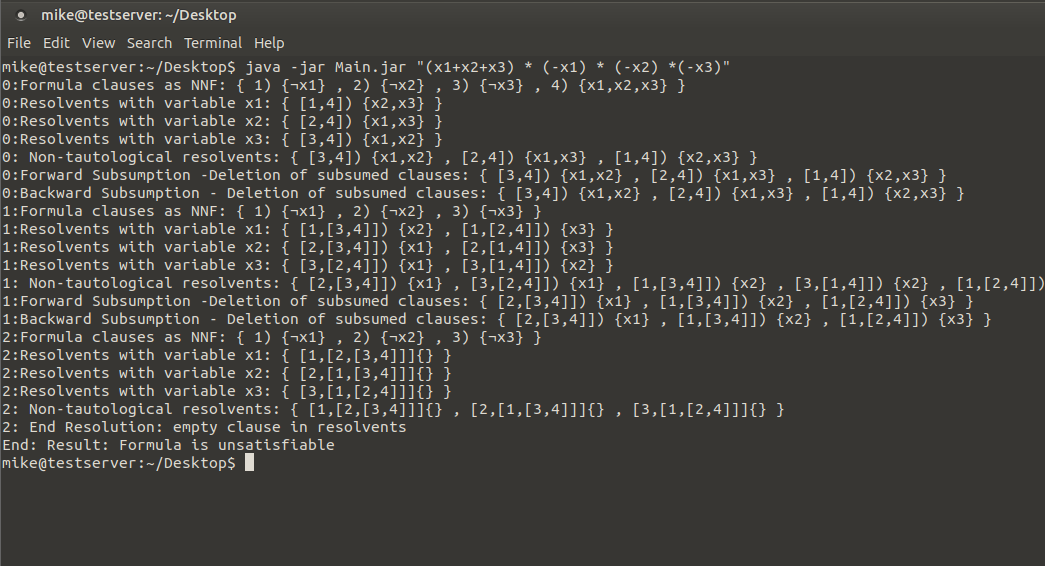
\includegraphics[width=14cm]{../Abbildungen/javaAusgabe.png}}
  \caption{Anwendung des Java-Programms mit Ausgabe}
  \label{fig1_1}
\end{figure}\\
Unabhängig von den Änderungen am logischen Ablauf wurde die Art des In- und Outputs ebenfalls abgewandelt. Das Tool liegt als jar-Datei auf dem Server und  arbeitet nun ausschließlich mit den Argumenten, die ihm bereits beim Start durch die API (siehe Punkt 4.4) übergeben werden. Danach werden keine zusätzlichen Parameter benötigt. \\
Die Teilschritte und das Endergebnis werden über die Kommandozeile ausgegeben, wo sie von der API gelesen und verarbeitet werden. In Abbildung 4.2 ist eine beispielhafte Anwendung des Java-Programms auf eine Formel zu sehen.\\

\section{Webserver}
Um die Webseite anzuzeigen wird sie über einen Webserver ausgegeben. Für dieses Projekt wurde ein Apache Webserver verwendet, es wäre aber problemlos möglich kleinere und ressourcenärmere Webserver zu implementieren. Der Webserver ist bei diesem Projekt von eher geringer Bedeutung, da React dynamische Webseiten erzeugt deren Inhalte nicht vom Server, sondern clientseitig berechnet werden. Der Server liefert lediglich den Programmiercode der Seiten, kann diesen jedoch selbst nicht oder nur teilweise interpretieren. \\
Aus diesem Grund sind für den Webserver in diesem Fall auch keine der üblichen Optimierungen notwendig. Sogar bei sehr großen Nutzerzahlen wird pro Anfrage nur ein sehr kleiner Aufwand entstehen. Da wie in 4.1 bereits erwähnt auch keine Zustände verwaltet werden müssen, besteht nur ein geringer Kommunikationsaufwand zwischen Nutzer und Server. Die Berechnung der Ergebnisse wird von der API und dem Java Programm durchgeführt. Die Anzeige der Ergebnisse wird wiederum von den Nutzergeräten erledigt. Pro Nutzer wird die Seite also nur einmal ausgeliefert und dann verwendet, bis die Seite neu geladen oder geschlossen wird.
\section{React Applikation}
Die React Applikation wurde mithilfe der Toolchain Create React App erstellt. Wie bereits in Kapitel 3 erwähnt, ist diese für derartige single-page Apps besonders gut geeignet. Dank Create React App sind alle nötigen Abhängigkeiten und Ordnerstrukturen von Projektbeginn an gegeben. \\
Bei Aufruf der Seite wird die Eingabemaske angezeigt:\\
\begin{figure}[htb]
     \centerline{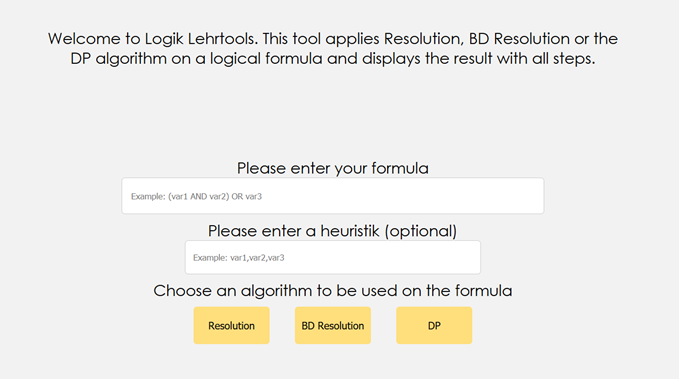
\includegraphics{../Abbildungen/eingabe.png}}
  \caption{Eingabemaske}
  \label{fig1_1}
\end{figure}\\
Dank JSX ähnelt der Code in React, beispielsweise für das Eingabefeld der Formel, dabei stark HTML:\\
\begin{figure}[htb]
     \centerline{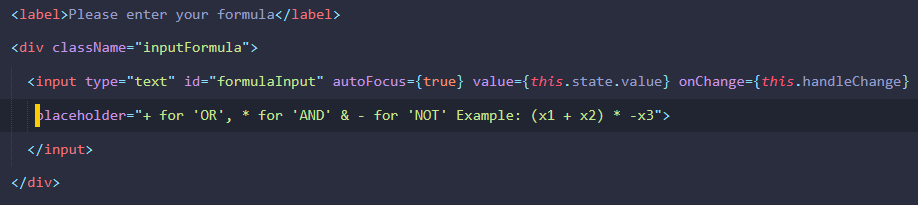
\includegraphics[width=14cm]{../Abbildungen/formulaInput.png}}
  \caption{Eingabefeld der Formel in JSX-Syntax}
  \label{fig1_1}
\end{figure}\\
Wie in Abbildung 4.3 zu erkennen ist, verfügt das Feld über einen Zustand 'this.state'. Dessen Wert wird bei Laden der Seite mit 'null' initialisiert. Die Funktion 'onChange', zu sehen in Abbildung 4.4, wird diesem Komponenten übergeben. Sie sorgt dafür, dass die vom Nutzer eingegebene Formel den neuen Wert von 'this.state.value' bildet. Dieser neue Wert wird gleichzeitig auch im Eingabefeld angezeigt.\\
\begin{figure}[htb]
     \centerline{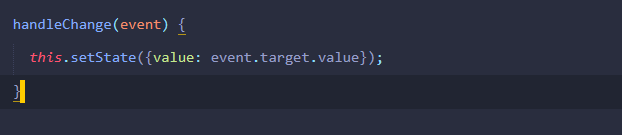
\includegraphics[width=14cm]{../Abbildungen/handleChange.png}}
  \caption{handleChange-Funktion}
  \label{fig1_1}
\end{figure}\\
Nachdem der User die Formel, eventuell eine Heuristik und den Algorithmus eingegeben hat, werden diese Angaben als Daten eines HTTP GET-Requests an den Server geschickt. Um diesen Request zu erzeugen wird Axios verwendet, ein schlanker und weit verbreiteter HTTP Client.
Dessen Installation und Nutzung ist dank der Modularität von React nur eine Sache von wenigen Zeilen. Nach Installation mittels eines Paketmanagers muss lediglich eine entsprechende Import-Zeile in der Javascript-Datei eingefügt werden. Anschließend kann der HTTP Client sofort mit allen Funktionen genutzt werden. \\
Als Ziel des GET-Requests wird ein anderer Port als der des Webservers verwendet, um die Daten an die Server API zu schicken. Die Daten werden im JSON-Format verschickt, da dieses von Axios unterstützt wird und die Daten von der API leicht ausgelesen werden können. In Abbildung 4.5 ist die Implementierung am Beispiel Resolution dargestellt.
\begin{figure}[H]
     \centerline{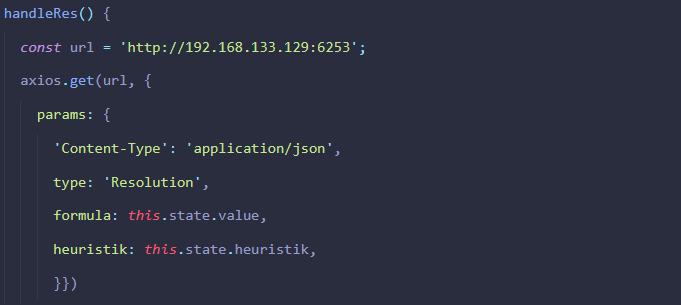
\includegraphics[width=14cm]{../Abbildungen/axiosResolution.png}}
  \caption{GET-Request für die Resolution}
  \label{fig1_1}
\end{figure}
Nach der Ergebnisberechnung erhält React eine Antwort mit den resultierenden Schritten als HTML-Tabelle. Mit Hilfe der Funktion 'dangerouslySetInnerHTML' ist React in der Lage diesen HTML-Code ohne weiteres in den bestehenden Code einzugliedern. Der abschreckende Name dieser Funktion wurde gewählt, da es generell gefährlich sein kann Nutzerinput ohne weiteres darzustellen. An dieser Stelle besteht keine solche Gefahr, da der Input von Teilen der Projektarchitektur generiert wurde.
Sobald die Daten erhalten und mittels 'dangerouslySetInnerHTML' angezeigt werden, entsteht auf der Webseite die erhaltene Tabelle (siehe Abbildung 4.6).\\
Um das Ergebnis auch kompakt darzustellen, untersucht React mittels String-matching das erhaltene Ergebnis und gibt je nach Fall an, ob die Formel erfüllbar ist oder nicht. Dazu wird Reacts Fähigkeit genutzt nicht nur HTML-Code, sondern sogar React-Code in Variablen speichern und direkt in bestehenden Code einzubauen. Die Methode, die das Ergebnis untersucht, erstellt eine entsprechende React-Komponente und übergibt diese an die passende Stelle im React-Code. \\
Um die Navigation für den Nutzer zu erleichtern, springt die Webseite nach dem Starten des Tools direkt an die Stelle, an der das Ergebnis angegeben wird. Dort gibt es durch einen entsprechenden Button die Möglichkeit zur Tabelle mit den Einzelschritten zu springen.
\begin{figure}[!htb]
     \centerline{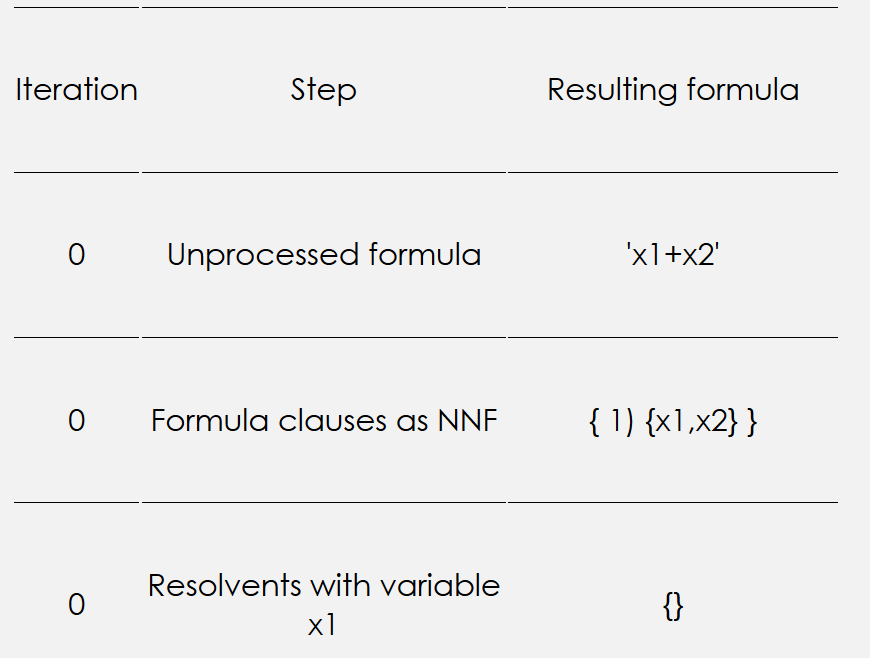
\includegraphics[width=14cm]{../Abbildungen/steps.png}}
  \caption{Ergebnistabelle}
  \label{fig1_1}
\end{figure}
\section{Server API}
Die API stellt die Schnittstelle zwischen Nutzereingabe und Java-Applikation dar. Dabei erfüllt sie drei Aufgaben: \\ 
1. Empfangen der eingegebenen Daten \\ 
2. Umwandlung dieser Daten in Startbefehle für die Applikation\\
3. Senden der Ergebnisse, die von der Applikation ausgegeben werden\\ 
Häufige Lösungen für Anforderungen dieser Art beinhalten das Nutzen des Webservers als Proxy, der bestimmte Anfragen an ein Framework weiterleitet. Da aber in diesem Fall die Anzahl der möglichen Fälle sehr gering ist, bot sich eine direktere und schmalere Lösung an.\\
Die Schnittstelle wurde daher über ein Python-Skript realisiert. Dieses bedient sich des Python „BaseHTTPServer“ Moduls, welches einen sehr kleinen HTTP-Server erzeugt. Der Server ist in der Lage auf einem angegebenen Port auf HTTP-Requests zu warten, diese zu verarbeiten und angepasste Antworten zu senden. \\
Für dieses Projekt muss lediglich auf den GET-Request, den React mittels Axios, versendet gewartet werden. Es sind keinerlei andere Anfragen zu erwarten, weshalb Anfragen die nicht in dieses Muster passen sofort verworfen werden können.\\
Handelt es sich um den erwarteten Request, werden die beinhalteten Daten aus JSON geparst und in einen Kommandozeilenbefehl verarbeitet. Dieser Befehl startet die Java-Applikation mit den erhaltenen Parametern.\\
Wie bereits in Punkt 4.1 erwähnt erzeugt die Applikation Ausgaben für die Komandozeile. Diese werden im Skript aufgefangen und können so als Datenset verwendet werden. Da React in der Lage ist HTML-Code zu empfangen und direkt zu verwenden, kann an dieser Stelle ein weiteres Verpacken der Daten in JSON vermieden werden. Stattdessen wird eine Tabelle aufgebaut, in der die Ergebnisse strukturiert und übersichtlich präsentiert werden können. Der HTML-Code wird nicht, wie möglicherweise zu erwarten wäre, mit dem Typ 'text/html' versehen. Stattdessen wird als Typ 'text/plain' angegeben. Grund dafür ist, dass so keine Notwendigkeit besteht, eine komplette HTML-Struktur aufzubauen. So ist es möglich nur den Code für die Tabelle zu senden, so dass er von der React Applikation ohne weiteres in die bereits bestehende Seite eingegliedert werden kann.
\section{Ausblick}
